\documentclass[10pt,twocolumn,preprint]{emulateapj}
\usepackage[english]{babel}
\usepackage{amsmath}

\newcommand{\bs}{\boldsymbol}
\newcommand{\diff}{{\mathrm d}}
\newcommand{\Cov}{\mathsf{C}}
\newcommand{\Fish}{\mathsf{F}}
\newcommand{\Cl}{\mathcal {C}}
\newcommand{\R}{\mathcal{R}}
\newcommand{\T}{\mathcal{T}}
\newcommand{\Msun}{M_\odot}


\shortauthors{Yu et al.} \shorttitle{CUBE}
\begin{document}
\title{CUBE: Compact Particle-Mesh $N$-body Algorithm}
\author{
Hao-Ran Yu$^{1,2}$,
Ue-Li Pen$^{2,3,4,5}$,
Xin Wang$^{2}$
}

\affil{
$^1$Kavli Institute for Astronomy and Astrophysics, Peking University, Beijing 100871, China\\
$^2$Canadian Institute for Theoretical Astrophysics, University of Toronto, Toronto, ON M5H 3H8 Canada\\
$^3$Dunlap Institute for Astronomy and Astrophysics, University of Toronto, Toronto, ON M5S 3H4, Canada\\
$^4$Canadian Institute for Advanced Research, CIFAR Program in Gravitation and Cosmology, Toronto, ON M5G 1Z8, Canada\\
$^5$Perimeter Institute for Theoretical Physics, Waterloo, ON N2L 2Y5, Canada
}

\email{haoran@cita.utoronto.ca}

\begin{abstract}
Cosmological large scale structure $N$-body simulations are computation-light but memory-heavy imbalanced problems in supercomputing. Traditional $N$-body simulation algorithms use at least 24-byte per particle in memory, where six 4-byte single precision real numbers keep track of each particle's phase space coordinate. This is usually the bottleneck of scaling-up of a $N$-body problem on modern supercomputers whose core/memory ratio is high. Here we present a parallel, memory-lite Particle-Mesh based $N$-body code, in which each particle can occupy as low as 6-byte memory. This is accomplished by storing only particles' relative location respect to a mesh-grid, and their velocity relative to a predictable distribution function. The remaining information is given by the ordering of particles, and a complimentary density field, which is negligible in memory space. Our numerical experiments show that this algorithm provides acceptable accuracy compared to traditional algorithm in cosmological simulations.

\end{abstract}

\keywords{}

\maketitle

\begin{figure}[t]
\centering
  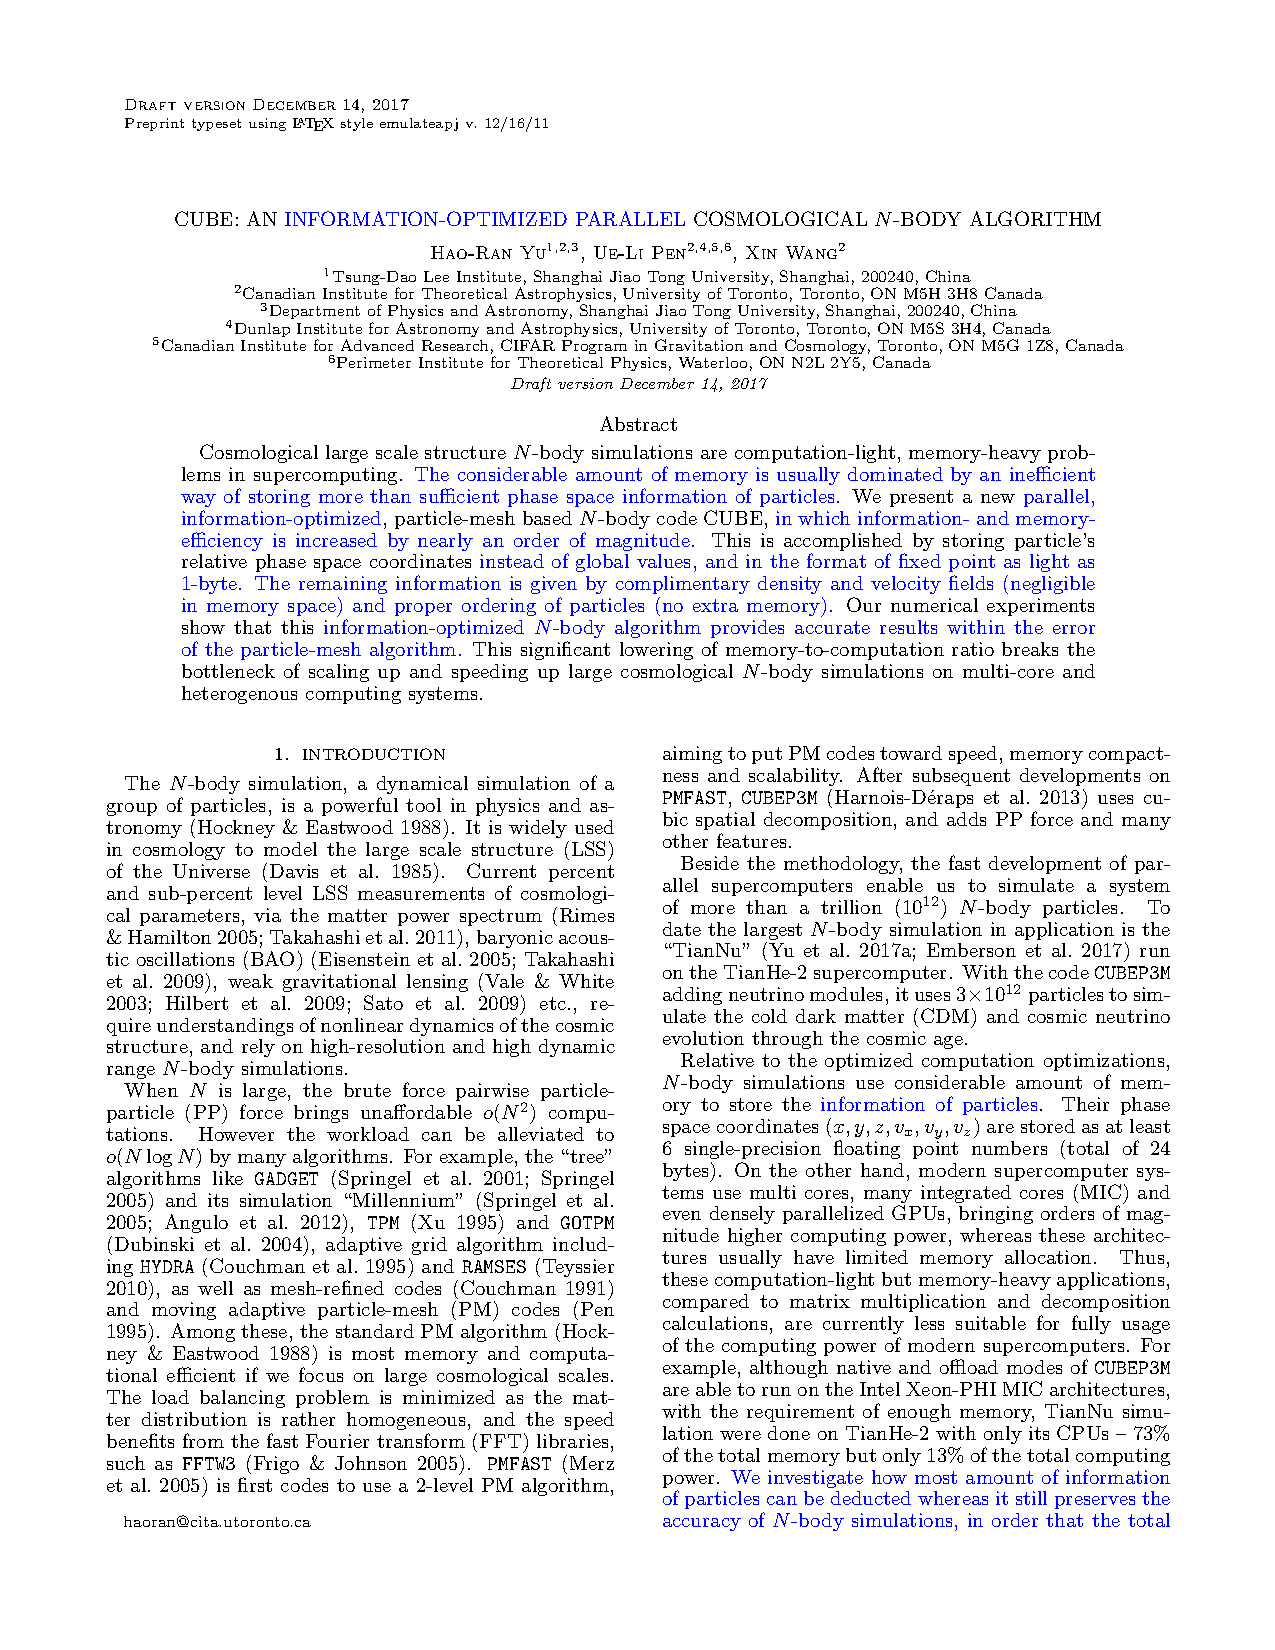
\includegraphics[width=0.95\linewidth]{ms_caf.pdf}
\end{figure}
\section{Introduction}
$N$-body simulation is a powerful tool to solve the highly nonlinear dynamic problems \citep{1988csup.book.....H}. It is widely used in cosmology to model the formation and evolution of the large scale structure (LSS). With the fast development of parallel supercomputers, we are able to simulate a system of more than a trillion ($10^{12}$) $N$-body particles. To date the largest $N$-body simulation in application is the ``TianNu'' simulation run on the TianHe-2 supercomputer by cosmological simulation code {\tt CUBEP3M} \citep{2013MNRAS.436..540H}. It uses nearly $3\times 10^{12}$ particles to simulate the cold dark matter (CDM) and cosmic neutrino evolution through the cosmic age. However {\tt CUBEP3M} and TianNu did not fully use TianHe-2's computing power -- 87\% of the computing power on TianHe-2 are given by the Intel Xeon-Phi coprocessors while they occupy only 27\% of the total memory. Although we accomplished preliminary works on developing native and offload modes of {\tt CUBEP3M} on Xeon-Phi many integrated core (MIC) architecture, the memory problem is still the bottle neck of scaling up the $N$-body problem on the heterogeneous architectures. Lower the memory usage per particle will solve this problem, and will also help the $N$-body problem development on GPUs, which are even more massive parallelized and memory limited. In this paper we present a $N$-body algorithm which uses as low as 6 byte per particle (here after we use ``bpp'' referring to ``byte per particle'') and show that it can give accurate cosmological LSS simulations. The algorithm is presented in \S 2, and a comparison between this method and traditional method is shown in \S 3. Discussions and conclusions are in \S 4.

\section{Algorithm}
The most memory consuming part of a $N$-body simulation is usually the phase space coordinates of each $N$-body particles -- 24 bpp (4 single precision real numbers) must be used to store each particles' position and velocity. A memory-lite parallel $N$-body code {\tt CUBEP3M} can use as low as 40 bpp in sacrificing the speed. This includes the phase coordinates (24 bpp) for particles in physical domain and buffered region, a linked list (4 bpp), and a global coarse mesh and local fine mesh. We attempt to replace the coordinates and linked list 24+4=28 bpp memory usage with a integer based storage, described as follows.

\subsection{Particle location storage}
Instead of storing the particle's global coordinates, we store its relative position respective to the coarse cell who contains the particle. We divide the coarse cell, in each dimension, evenly into $2^8=256$ bins, and we use a 1-byte integer (with range 0 to 255 or -128 to 127) to show which bin it locates in this dimension. Next, global locations of particles are given by cell-ordered format in memory space, and a complimentary number count of particle number in this coarse mesh (coarse density field) will give complete information of particle distribution in cells. Since the this field is usually coarser than particle distribution, it takes negligible memory. This coarse density field can be further compressed into 1-byte integer format, such that a 1-byte unsigned integer show the particle number in this coarse cell in range 0 to 255. In the densest cells (rarely happened) where there are $\ge 255$ particles, we can just write 255, and write the actual number as a 4-byte integer in another file. In a simulation with volume $L^3$ and $N_c^3$ coarse cells, particle positions are stored with a precision of $L/(256N_c)$, which is usually 10 times finer than the force resolution.

\subsection{Particle velocity storage}\label{s.velocity}
Velocities, in each dimension, are compressed to 2-byte integers representing their index within a histogram containing $2^{16}$ equally spaced bins ranging from $-v_{\rm max}$ to $v_{\rm max}$, where $v_{\rm max}$ is the maximum absolute particle velocity. $v_{\rm max}$ can be derived from either computation or prediction. We prefer the latter case. In cosmological simulations, velocity distribution of matter fluids can be predicted by linear theory, given a model and redshift $z$ (time of the simulation). Then by any time step, we have a cumulative distribution function (CDF) $F(|\bs{v}|)$ of particles' velocity (see appendix A). We, instead, equally divide the $y$-axis of this CDF into $2^{16}$ bins, and the 2-byte integer shows which velocity bin the particle locates, in each dimension. This step does finer sampling on low-velocity end in velocity space and increases the simulation accuracy. This CDF may introduce velocity cutoffs, that particle cannot exceed some certain $\bs{v}_{\rm max}(z)$ given by the model. This process prevents the nonphysical scattering behaviours of particles, which do not exist in fluids. Practically, simulation results are very insensitive to the choice of velocity distribution. Even a top-hat distribution in range $-v_{\rm max}$ to $v_{\rm max}$ give accurate results. One can just assume a Gaussian distribution and whose standard deviation is given by the model and redshift $\sigma(\bs{\theta},z)$. Proper choice of model only optimizes the velocity space sampling, but does not affect the physics.

\begin{figure}[t]
\centering
  \includegraphics[width=0.95\linewidth]{fig_tile.pdf}
 \caption{Spacial decomposition.}
\label{fig.tile}
\end{figure}

\subsection{Spacial decomposition}
{\tt CUBE} uses cubic decomposition structures. The global simulation volume is decomposed into ${\tt nn}^3$ cubic sub-volumes, and each of these are assigned to a coarray {\it image}\footnote{Images are the concept of computing nodes or MPI tasks in Coarray Fortran. We use this terminology in this paper.}. Inside of an image, the sub-volume is further decomposed into ${\tt nnt}^3$ cubic {\it tiles}. Each tile is surrounded by a {\it buffer} region which is usually ${\tt ncb}$ coarse cells thick. The buffer is designed for two reasons: (1) computing the fine mesh force, whose cut-off ${\tt nforce\_cutoff}\leq{\tt ncb}$, and (2) collecting all possible particles travelling from a tiles buffer region to its center, {\it physical} region. Thus, a integer-based coarse mesh density is defined as
\begin{equation*}
{\tt integer(1)\ rho\_c(nex,nex,nex,nnt,nnt,nnt)[nn,nn,*]}\\
\end{equation*}
where ${\tt nex}={\tt nt}+2{\tt ncb}$ covers the buffer region on both sides, {\tt nnt} is the tile dimemsions, and {\tt nn} is the image {\it codimensions}\footnote{Coarray Fortran concept. Codimensions can do communications between images.}. Particles' phase coordinates {\tt x} and {\tt v} are copied between tiles and images, when necessary. Figure \ref{fig.tile} shows the spacial decomposition in a 2-dimensional analogy, with ${\tt nn=2}$ and ${\tt nnt=2}$.

\begin{figure}[t]
\begin{verbatim}


    program CUBE
      call initialize
      call particle_initialize
      sync all
      call buffer_density
      call buffer_x
      call buffer_v
      do
        call timestep
        call update_x
        call buffer_density
        call buffer_x
        call PM ! update_v
        call buffer_v
        if(checkpoint_step) then
           call checkpoint
           if (final_step) exit
        endif
      enddo
      call finalize
    endprogram
\end{verbatim}
\caption{Overall structure of {\tt CUBE}.}
\label{fig.code}
\end{figure}

\subsection{Code overview}
By using the previous compact format storage, we modified the {\tt CUBEP3M} and utilized it in the outputs TianNu simulation. On average, 9.125 bpp is used for all outputs and saves 62 \% hard drive space on Tianhe-2. The compact version of {\tt CUBEP3M}, named {\tt CUBE}, accomplished the compact format in memory, and the code keeps only integer format for storing particles' phase space coordinates. {\tt CUBE} is written in Coarray Fortran, where the coarray features are used to do MPI communications. Here we review the methodology of solving this integer based $N$-body problem. Like its predecessor {\tt CUBEP3M}, {\tt CUBE} uses two-level mesh grids for solving the Poisson equations. The advantages of this are described in \cite{2013MNRAS.436..540H}.

Figure \ref{fig.code} shows the overall structure of the code. Subroutine {\tt initialize} creates necessary FFT plans and read in configuration files telling the program at which redshifts we need to do checkpoints, halofinds, or stop the simulation. Force kernels are also created or read in here. In {\tt particle\_initialize}, for each image, we read in initial positions and velocities in the compressed format.  A initial condition generator is also written in the compressed format (see Appendix B). When this step is done by all images (synchronized by ``{\tt sync all}'', which is equivalent to a {\tt mpi\_barrier}), the density fields {\tt rho\_c} are buffered between tiles (communications between images are needed) by subroutine {\tt buffer\_density}. Then, particles' phase space coordinates {\tt x} and {\tt v} are also buffered, by {\tt buffer\_x} and {\tt buffer\_v} respectively. In these steps, {\tt x} and {\tt v}'s ordering is changed according to the updated {\tt rho\_c}.

In each iteration of the main loop, we firstly call {\tt timestep}, where a increment of time {\tt dt} is controlled by particles' maximum velocities, accelerations, and cosmic expansions. According to {\tt dt}, subroutine {\tt update\_x} updates the positions of particles in a ``{\it gather}'' algorithm. ${\tt x}={\tt x}+{\tt v}*{\tt dt}$ is executed twice, first time to determine a updated density field on the tile, {\tt rho\_c\_new}, and second time to generate a new particle list {\tt x\_new} and {\tt v\_new} on the tile. The reason for this repeated execution is the dependence of {\tt x\_new} and {\tt v\_new}'s value and ordering on both the old {\tt x}, {\tt v} and the new {\tt rho\_c\_new}. However, ${\tt x}={\tt x}+{\tt v}*{\tt dt}$ scales as $o(N)$ and is computational inexpensive. Although {\tt x\_new} and {\tt v\_new} arrays take extra memory, they do not appear simultaneously for multiple tiles, and compared to {\tt x} and {\tt v}, the extra memory overhead is by factor of $1/{\tt nnt}^3$. This requires the ``gather'' algorithm to move particles\footnote{In contrast, {\tt CUBEP3M} uses a ``{\it scatter}'' algorithm.} -- as we synchronize the correct \{{\tt rho\_c}, {\tt x}, {\tt v}\} in the buffer region of each tile, and the particles in the extended (physical+buffer) region are a superset of particles locating in the physical region in the next time step, given that ${\tt v}*{\tt dt}$ is not greater than the buffer depth. In {\tt update\_x}, \{{\tt rho\_c\_new}, {\tt x\_new}, {\tt v\_new}\} can be set to collect only the physical region of the tile, with the rest of this subset discarded. At the end, \{{\tt rho\_c}, {\tt x}, {\tt v}\} is replaced by \{{\tt rho\_c\_new}, {\tt x\_new}, {\tt v\_new}\}, and the memory of latter is freed up.

Next, {\tt buffer\_density} and {\tt buffer\_x} are called again to synchronize the updated particle positions in order that tile-based local fine forces are computed correctly.

A standard particle-mesh scheme is then performed in the {\tt PM} subroutine. First, by looping over tiles, fine force is calculated and velocities are updated on the physical region of each tile. The memory overhead of fine-mesh arrays are well controlled by $1/{\tt nnt}^3$. Next, global coarse force is solved by using a coarser (usually by factor of 4) mesh by dimensional splitting -- a distributed-memory cubic decomposed 3D coarse density field is interpolated by particles, and we Fourier transform data in consecutive three dimensions with global transposition in between (known as the pencil decomposition). After the multiplication of force kernels, the inverse transform takes place to get the cubic distributed coarse force field, upon which velocities are updated again. The memory usage of coarse arrays are negligible. An optional particle-particle (PP) force can be called to increase the force resolution and the velocities are updated last time according to this. As discussed in \S\ref{s.velocity}, updating velocities use model predicted velocity distribution, thus ${\tt v}={\tt v}+{\tt dv}$ is executed only once, scaling directly to the velocity distribution of the next time step ${\tt d}+{\tt dt}$. During each of these force calculations, maximum accelerations are collected serving for the {\tt timestep} in the next iteration, controlling next {\tt dt}.

By far, particle velocities in the physical regions of each tile are updated. Particle locations in the buffer regions has updated before {\tt PM} and remained unchanged. So we simply call {\tt buffer\_v} again, such that the {\tt update\_x} in the next iteration will be done correctly.

If a desired redshift is reached, we call {\tt checkpoint} and/or exit the main loop. The corresponding logical variables are controlled in {\tt timestep}. Finally, in {\tt finalize} subroutine we destroy all the FFT plans and finish up any timing or statistics taken in the simulation.

\begin{figure}[t]
\centering
  \includegraphics[width=0.95\linewidth]{ddsp_pcdf_256_box80.pdf}
 \caption{Displacement.}
\label{fig.dsp}
\end{figure}

\subsection{Memory layout}
Here we summarize the memory usage in unit of bpp (byte per particle).

\section{Results}
We use the same initial conditions, and use {\tt CUBEP3M} and {\tt CUBE} to simulate the large scale structure formation separately and compare their results.

Results of {\tt izipx=1}

Results of {\tt izipx=2}

\begin{figure}[h]
\begin{verbatim}
















\end{verbatim}

\caption{Power spectrum differential plot}
\label{fig.power}
\end{figure}

\section{Discussion and Conclusion}
Cosmological simulation, PM method.

PID.

Summarize memory.

Phi, GPU.


\clearpage

\appendix
\section{A. Velocity distribution function}
To optimize the storage of the velocity field, we need to estimate the velocity dispersion at each snapshot. At non-linear scale, the velocity distribution function is surely non-Gaussian. However, to the first order approximation, we simply assume it as Gaussian and characterized by the variance
\begin{eqnarray}
\sigma_v = \frac{1}{3}  (a H f D)^2 \int d^3q \frac{P_{L}(q)}{q^2} 
\end{eqnarray}
where $a(z)$ is the scale factor, $H(z)$ the Hubble parameter, $D$ is the linear growth factor, $f=d \ln D/d\ln a$, 
and $P_L(k)$ is the linear power spectrum of density contrast at redshift zero. 

 

\section{B. Initial condition generator}


\acknowledgements
Thanks.

\bibliographystyle{hapj}
\bibliography{haoran_ref}

\end{document}
